\documentclass[a4paper,10pt]{article}

%A Few Useful Packages
\usepackage{marvosym}
\usepackage{fontspec} 					%for loading fonts
\usepackage{xunicode,xltxtra,url,parskip} 	%other packages for formatting
\RequirePackage{color,graphicx}
\usepackage[usenames,dvipsnames]{xcolor}
\usepackage[big]{layaureo} 				%better formatting of the A4 page
% an alternative to Layaureo can be ** \usepackage{fullpage} **
\usepackage{supertabular} 				%for Grades
\usepackage{titlesec}					%custom \section
\usepackage{comment}
\usepackage{multirow}
\usepackage{float}
\usepackage{tabularx}
\usepackage{xcolor}

%Setup hyperref package, and colours for links
\usepackage{hyperref}
\definecolor{linkcolour}{rgb}{0,0.2,0.6}
\hypersetup{colorlinks,breaklinks,urlcolor=linkcolour, linkcolor=linkcolour}

%FONTS
\defaultfontfeatures{Mapping=tex-text}
%\setmainfont[SmallCapsFont = Fontin SmallCaps]{Fontin}
%%% modified for Karol Kozioł for ShareLaTeX use
\setmainfont[
SmallCapsFont = Fontin-SmallCaps.otf,
BoldFont = Fontin-Bold.otf,
ItalicFont = Fontin-Italic.otf
]
{Fontin.otf}
%%%

%CV Sections inspired by: 
%http://stefano.italians.nl/archives/26
\titleformat{\section}{\Large\scshape\raggedright}{}{0em}{}[\titlerule]
\titlespacing{\section}{0pt}{3pt}{3pt}
%Tweak a bit the top margin
%\addtolength{\voffset}{-1.3cm}

%Italian hyphenation for the word: ''corporations''
\hyphenation{im-pre-se}

%-------------WATERMARK TEST [**not part of a CV**]---------------
\usepackage[absolute]{textpos}

\setlength{\TPHorizModule}{30mm}
\setlength{\TPVertModule}{\TPHorizModule}
\textblockorigin{2mm}{0.65\paperheight}
\setlength{\parindent}{0pt}

\addtolength{\oddsidemargin}{-.675in}
\addtolength{\evensidemargin}{-.675in}
\addtolength{\textwidth}{1.35in}

\addtolength{\topmargin}{-.675in}
\addtolength{\textheight}{1.75in}

% define "struts", as suggested by Claudio Beccari in
%    a piece in TeX and TUG News, Vol. 2, 1993.
\newcommand\Tstrut{\rule{0pt}{3ex}}         % = `top' strut
\newcommand\Bstrut{\rule[-1.5ex]{0pt}{0pt}}   % = `bottom' strut

\definecolor{myblue}{RGB}{51,132,204}


%--------------------BEGIN DOCUMENT----------------------
\begin{document}

%WATERMARK TEST [**not part of a CV**]---------------
%\font\wm=''Baskerville:color=787878'' at 8pt
%\font\wmweb=''Baskerville:color=FF1493'' at 8pt
%{\wm 
%	\begin{textblock}{1}(0,0)
%		\rotatebox{-90}{\parbox{500mm}{
%			Typeset by Alessandro Plasmati with \XeTeX\  \today\ for 
%			{\wmweb \href{http://www.aleplasmati.comuv.com}{aleplasmati.comuv.com}}
%		}
%	}
%	\end{textblock}
%}

\pagestyle{empty} % non-numbered pages

%\font\fb=''[cmr10]'' %for use with \LaTeX command

%--------------------TITLE-------------

\begin{table}[H]
\centering

\begin{tabular}{c | l }
  \multirow{4}{*}{\Huge David Laredo} & Computer scientist skilled in the fields of mechanical engineering, machine\\ 
  & learning and statistics. I have led or supervised the development of more  \\
  & than three novel methods for the application of machine learning to \\
  \textcolor{myblue}{\textbf{Senior Research Assistant}} & engineering problems. 
\end{tabular}

\end{table}

\vspace{-2.5ex}
\begin{table}[H]
\centering

\begin{tabular}{r l | r l | r l | r l}
 
\includegraphics[scale=0.017]{icons/email.jpeg} \hspace{-1.3em} & myemail@gmail.com & 
 
\includegraphics[scale=0.015]{icons/phone.jpeg} \hspace{-1.3em} & +52 1 0123456789 & 
 
\includegraphics[scale=0.015]{icons/url.jpeg} \hspace{-1.3em} & linkedin.com/in/yourlinkedin/ & 
 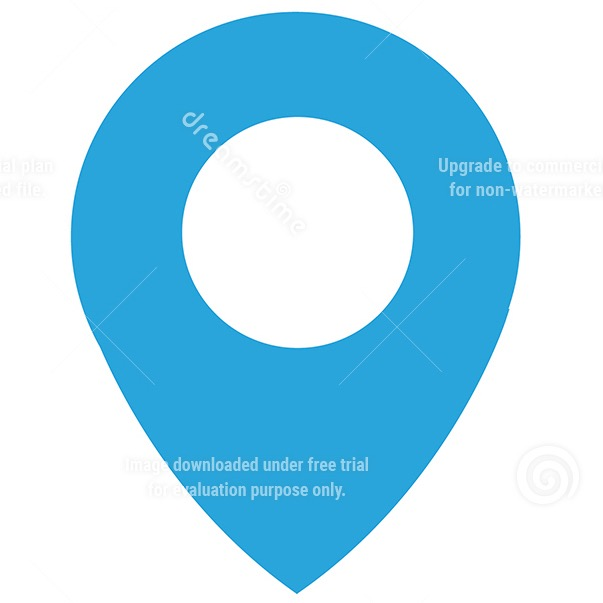
\includegraphics[scale=0.015]{icons/location.jpeg} \hspace{-1.3em} & Some place here \Tstrut\Bstrut\\
\end{tabular}

\vspace{-2.5em}
\noindent\hrulefill
\vspace{1em}

\end{table}



%--------------------SECTIONS-----------------------------------

\begin{minipage}[H]{0.7\textwidth}%

%Section: Work Experience at the top
\section{Experience}
\textbf{Senior Research Assistant, Summer 2017 - Summer 2019}\\
\emph{University of California, Merced}
\begin{itemize}
\item Led a team that developed an \textbf{algorithm for the automatic selection of neural network models}. Algorithm works for classification and regression problems. The 						obtained models yield an accuracy of up to 95\%.
\item Led a team that developed a \textbf{machine learning method for estimating the remaining useful life (RUL) of jet engines}. The method predicts the RUL of 75\% of the 							tested engines with a confidence of \pm 5 cycles.
\item Developed a \textbf{machine learning method to detect faults in an HVAC system}. The system performs online classification of faults in the system with an accuracy of 80\%.
\end{itemize}

\textbf{Firmware Engineer, Fall 2015 - Fall 2016}\\
\emph{Intel, Guadalajara}
\begin{itemize}
\item Responsible of BIOS development for the PCH module: debugging and implementation of new features.
\item Implemented new BIOS features for Intel's micro-server SoC such as IO Memory, Ethernet, IO devices.
\item Implemented support for wake-on-LAN and for the use of high IO memory on Intel's Denverton platform.
\end{itemize}

\textbf{Business Application Developer, Fall 2012 - Fall 2013}\\
\emph{Anzen Consultancy, Mexico City}
\begin{itemize}
\item Front end application developer for Citibank in Mexico.
\item Implemented new features for Citi's web banking system such as balance inquiries and account statements.
\end{itemize}


%Section: Education
\section{Education}

\textbf{M.S. in Mechanical Engineering - GPA:3.6}\\
\emph{University of California - Merced, Fall 2016 - Fall 2019}\\
Thesis: ``Application of Deep Learning Methods in the Treatment of Mechanical Engineering Problems.''\\
Relevant Coursework: Machine Learning, Controls, Dynamics, Numerical Analysis.

\textbf{M.S. in Computer Science - GPA:3.5}\\
\emph{CINVESTAV-IPN, Fall 2013 - Fall 2015}\\
Thesis: ``A Continuation Method for Solving Mixed-Integer Multi-objective Optimization Problems.''\\
Relevant Coursework: Numerical Optimization, Statistics, Algorithm Design, Evolutionary Algorithms.

\textbf{B.E. in Computer Engineering - GPA:3.0}\\
\emph{ESCOM-IPN, Fall 2018 - Fall 2012}\\
Relevant Coursework: Object Oriented Programming, Database Design, Algorithm Design, Software Engineering.
\end{minipage}%
\begin{minipage}[H]{0.2\textwidth}%

\section{Computer Skills}
\begin{tabular}{rl}
Proficient:& Python, \textsc{SQL}, \textsc{C/C++}, Java, Tensorflow, Scipy, Matlab, Excel, Powerpoint, Latex\\
Intermediate:& R, \textsc{UNIX}/Linux, Simulink, Javascript, Fortran\\
\end{tabular}

%Section: Languages
\section{Languages}
\begin{tabular}{rl}
\textsc{Spanish:}&Native\\
\textsc{English:}&Proficient/Fluent\\
\end{tabular}

\end{minipage}%

\end{document}
